\chapter{Certification}
This chapter focuses on the process and the steps required to obtain the certification of HUGO to be used for the research purpose of testing the aeroelastic effects of high aspect ratio wings. In the first section (cite) the classification process is described that places HUGO into a type class category. Following the assessment of flight class, the certification for a Design Organisational Approval (DOA) is covered, where the different wings' and tail designs are considered.

\section{Type Certificate}

\section{Design Organisational Approval (DOA)}
For the certification procedure of an aircraft, the competent authority in Europe, EASA, requires extensive documentation and validation procedures of the design. For this stage of the UAV design, several EASA-imposed operational restrictions must be considered, including the applicable airworthiness class and the permitted operational environment.

Certification of an aircraft, or of modifications brought to it, involves contacting EASA so they can take the following steps\footnote{\href{https://www.easa.europa.eu/en/domains/aircraft-products/aircraft-certification?}{EASA Aircraft Certification}(accessed on 04.05.2026)}:

\begin{itemize}
    \item Technical familiarisation and certification basis
    \item Establishment of the certification programme
    \item Compliance demonstration
    \item Technical closure and issue of approval
\end{itemize}

Costs involved in this process and the time required for analysis of the design are not well defined, but can range from months to years, depending on the complexity of the idea. This conflicts with HUGOs' mission, whitch requires it to be able to fly with new modifications to its structure almost every time. Since the recertification process is applied for any modifications, this would result in an excess of downtime of the UAV, loss in revenue, \textcolor{red}{A VERY SAD SULTAN} and ultimately loss of purpose of such a platform.

EASA classifies that a new recertification for the aircraft is required each time a change is implemented, such changes further falling into 2 types: \textbf{Minor changes} and  \textbf{Major Changes}. A \textbf{Minor change} is classified as any type of modification that does not show any appreciable effect on weight, structural strength, reliability and other specifications \footnote{\href{https://www.easa.europa.eu/en/document-library/easy-access-rules/online-publications/easy-access-rules-initial-airworthiness-and?page=10#_Toc256000121}{Initial Airworthiness and Environmental Protection}(accessed on 06.05.2026)}. Under the DOA, there is also the possibility to conduct research, which is not scrutinised by EASA when done within the certification limits. \todo{cite email} 

Modifications made to HUGO for each mission will require EASA recertification, as they fall under the \textbf{Major changes} category. This condition directly conflicts with the modularity requirement of HUGO. By having a modular configuration, HUGO will be susceptible to regular structural changes of the wings, which are considered major modifications by EASA.  To bypass this process, or to the very least to make it shorter, the team behind HUGO can apply for a DOA \footnote{\label{DOA_site}\href{https://www.easa.europa.eu/en/domains/aircraft-products/design-organisations/design-organisations-approvals}{Design Organisations Approvals}(accessed on 05.06.2026)}.

A  DOA is a certification that permits the holder or organisation to perform the certification process internally, bypassing the long waits and costs imposed by EASA, leaving only the approval of the documentation to the discretion of the certification authority, EASA. This will be very useful for HUGO, as the DOA will permit the design team to internally bring and approve of modifications that fall under the \textbf{Minor} category. Regarding the modifications brought to the wings platform, the DOA permits us to categorise this procedure as a research procedure, excluding the need for recertifications and EASA interactions \todo{cite the email}.

When it comes to the implementation of the DOA, after consultations with an EASA employee, it was determined that inside the organisation, there has to be a specific department that will obtain the permission from EASA to supervise the changes brought to HUGO and their validation. For this design, a department formed of 3 people will be enough to supervise the design process, perform the required validation and ensure compliance with EASA. Pricing of the DOA is set at \EUR{10 170}, for the initial certification, and then EASA charges a 12-month billing cycle fee, to continue oversight of the approved organisation, set at \EUR{11050} \footnote{\hyperlink{https://eur-lex.europa.eu/eli/reg_impl/2025/2347/oj}{EASA Prices}(accessed on 08.05.2026)}.

\textbf{\textcolor{red}{THIS IS OFFICIALLY MY RESIGNATION FROM THE WRITING AND RESEARCHING PART CONCERNING ANYTHING THAT HAS TO DO WITH EASA}}


%while changes falling under the \textbf{Major} category still require approval from EASA. With this recognition, EASA only requires the validation proof and data to verify them and give the final decision\footnote{\href{https://eur-lex.europa.eu/legal-content/EN/TXT/?uri=CELEX\%3A02012R0748-20230825}{EASA DOA Documentation} (accessed on 06.05.2026).}. In terms of operational impediment, it will require users to submit their test beds in advance, with at least TBD.

% The process is applied each time a "major" modification (a defined by EASA in \todo{cite EASA major and minor modifications}) is applied to the aircraft. This condition directly conflicts with the modularity requirement of HUGO. By having a modular configuration, HUGO will be susceptible to regular structural changes of the wings, which are considered major modifications by EASA and are subject to recertification. 

% DOA is a certification that allows the organisation a certain degree of freedom when it comes to certifications and decisions of some aspects of design and operations. 
% %\subsection{DOA Implications}


%\subsection{Application Procedure and Documentation}

\begin{comment}
\section{Requirements following from CS-23 Amendment 4}
This Section describes the requirements for aerobatic aircraft following from Acceptable Means of Compliance (AMCs) detailed in EASA CS-23 Amendment 4 \cite{EASA_CS23_Amendment4}.

\subsection{Proof of Structure}
According to the AMCs for CS-23 aircraft, demonstration of compliance shall be achieved predominantly with the use of flight tests. However, analyses including FEM models are also acceptable, so long as their reliability for the certified structure is proven, and they are supplemented by a comparison of other methods regarded as sufficiently accurate and applicable. A strength test programme shall additionally be established for the wing, wing carry through, fuselage and empennage structures (e. g. via ultimate load testing). 

To account for material and production variability, a test correction factor $T_f$ shall be applied to each test based on the coefficient of variation $c_v$ provided by the manufacturer for a given product (see: \autoref{tab:test_factors}). The $c_v$ is defined by \autoref{eq:coefficient_of_variation} for a population with mean $M$ and standard deviation $\sigma$ \cite[p. 2-C-2]{EASA_CS23_Amendment4}.

\begin{equation}
\label{eq:coefficient_of_variation}
c_v=100\cdot\frac{\sigma}{M}\hspace{0.1cm}[\%]
\end{equation}

\begin{table}[H]
    \centering
    \caption{Test Factor $T_f$ vs. Coefficient of Variation $c_v$ (adapted from \cite[p. 2-C-2]{EASA_CS23_Amendment4})}
    \begin{tabular}{|c||c|c|c|c|c|c|c|c|c|c|}
    \hline
         $c_v$ [\%] & 5 & 6 & 7 & 8 & 9 & 10 & 12 & 14 & 15 & 20 \\\hline
         $T_f$ [-] & 1.00 & 1.03 & 1.06 & 1.10 & 1.12 & 1.15 & 1.22 & 1.30 & 1.33 & 1.55 \\ \hline
    \end{tabular}
    \label{tab:test_factors}
\end{table}

\subsection{Gust Load Factors}

\subsection{Unsymmetrical Flight Conditions}
The approach towards establishing the loads due to unsymmetric manoeuvres

\subsection{Flight Performance}
Each performance requirement shall be met at a combination of weight and CG location corresponding to the loading conditions for which HUGO is to be certified \cite{EASA_CS23_Amendment4}. According to EASA, the applicable methods of demonstrating compliance are tests upon an aircraft of HUGO's type or calculations based on, and equal in accuracy to, the results of testing, followed by systematic investigation of possible combinations of weight and CG.

An overview of acceptable general tolerances allowed in flight tests is presented in \autoref{tab:test_tolerances}
\todo[inline]{Add CG to nomenclature}
\begin{table}[H]
    \centering
    \caption{General Tolerances Allowed in Flight Tests (adapted from \cite{EASA_CS23_Amendment4})}
    \begin{tabular}{|c|c|}
        \hline
        \textbf{Item} &  \textbf{Tolerance} \\\hline\hline
         Weight & $+5\%,-10\%$ \\\hline
         Critical Items affected by Weight & $+5\%,-1\%$ \\ \hline
         Total CG travel & $\pm7\%$\\ \hline
    \end{tabular}
    \label{tab:test_tolerances}
\end{table}

\end{comment}



\section{V-n diagram}
The flight envelope of the HUGO aircraft in symmetric flight is based on CS-23 airworthiness requirements for aerobatic aircraft, as outlined in  \cite{EASA_CS23_Am3_2012}. Therefore, the positive limit manoeuvre load factor is 6.0, and the negative limit manoeuvre load factor is -3.0. 

\begin{figure}[H]
    \centering
    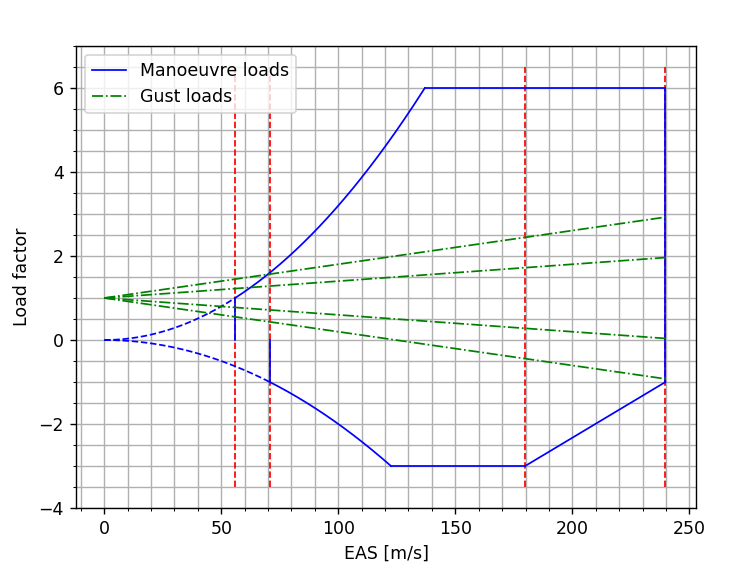
\includegraphics[width=1.0\linewidth]{figures/V-n_diagram.png}
    \caption{V-n diagram for the aircraft of $50kg$ mass $2.0m$ span, $AR=25.0$, cruise altitude of $5500.0m$, cruise Mach number of $0.75$, compliant with CS-23 aerobatic category requirements}
    \label{fig:V-n_diagram}
\end{figure}